\documentclass{beamer}
\usepackage{amsfonts, amsmath, graphicx, verbatim, graphicx, hyperref,
  color, caption, subcaption}
\definecolor{UNBlue}{RGB}{91, 146, 229}
\setbeamercolor{structure}{fg=UNBlue}
\newcommand\Fontvi{\fontsize{6.5}{7.2}\selectfont}
\usetheme{Warsaw}

\title{Flag Aggregation and Much More ...}
\author{\it Michael C. J. Kao}
\institute{Food and Agriculture Organization \\ of the United Nations}
\date{}

\AtBeginSection[]
{
  \begin{frame}<beamer>
    \frametitle{Outline for section \thesection}
    \tableofcontents[currentsection]
  \end{frame}
}

\begin{document}

\frame{
  \titlepage
  \centering
  
\includegraphics[scale = 0.2]{fao_logo.png}
}

\frame{
  \frametitle{Outline}
  \tableofcontents
}


\section{Introduction}

\frame{
\vfill
\begin{figure}
        \centering
        \begin{subfigure}[c]{0.5\textwidth}
                
\includegraphics[width=\textwidth]{all_flags.png}
                %% \caption{A gull}
                %% \label{fig:gull}
        \end{subfigure}%
        ~ %add desired spacing between images, e. g. ~, \quad, \qquad, \hfill etc.
          %(or a blank line to force the subfigure onto a new line)
        \begin{subfigure}[c]{0.1\textwidth}
                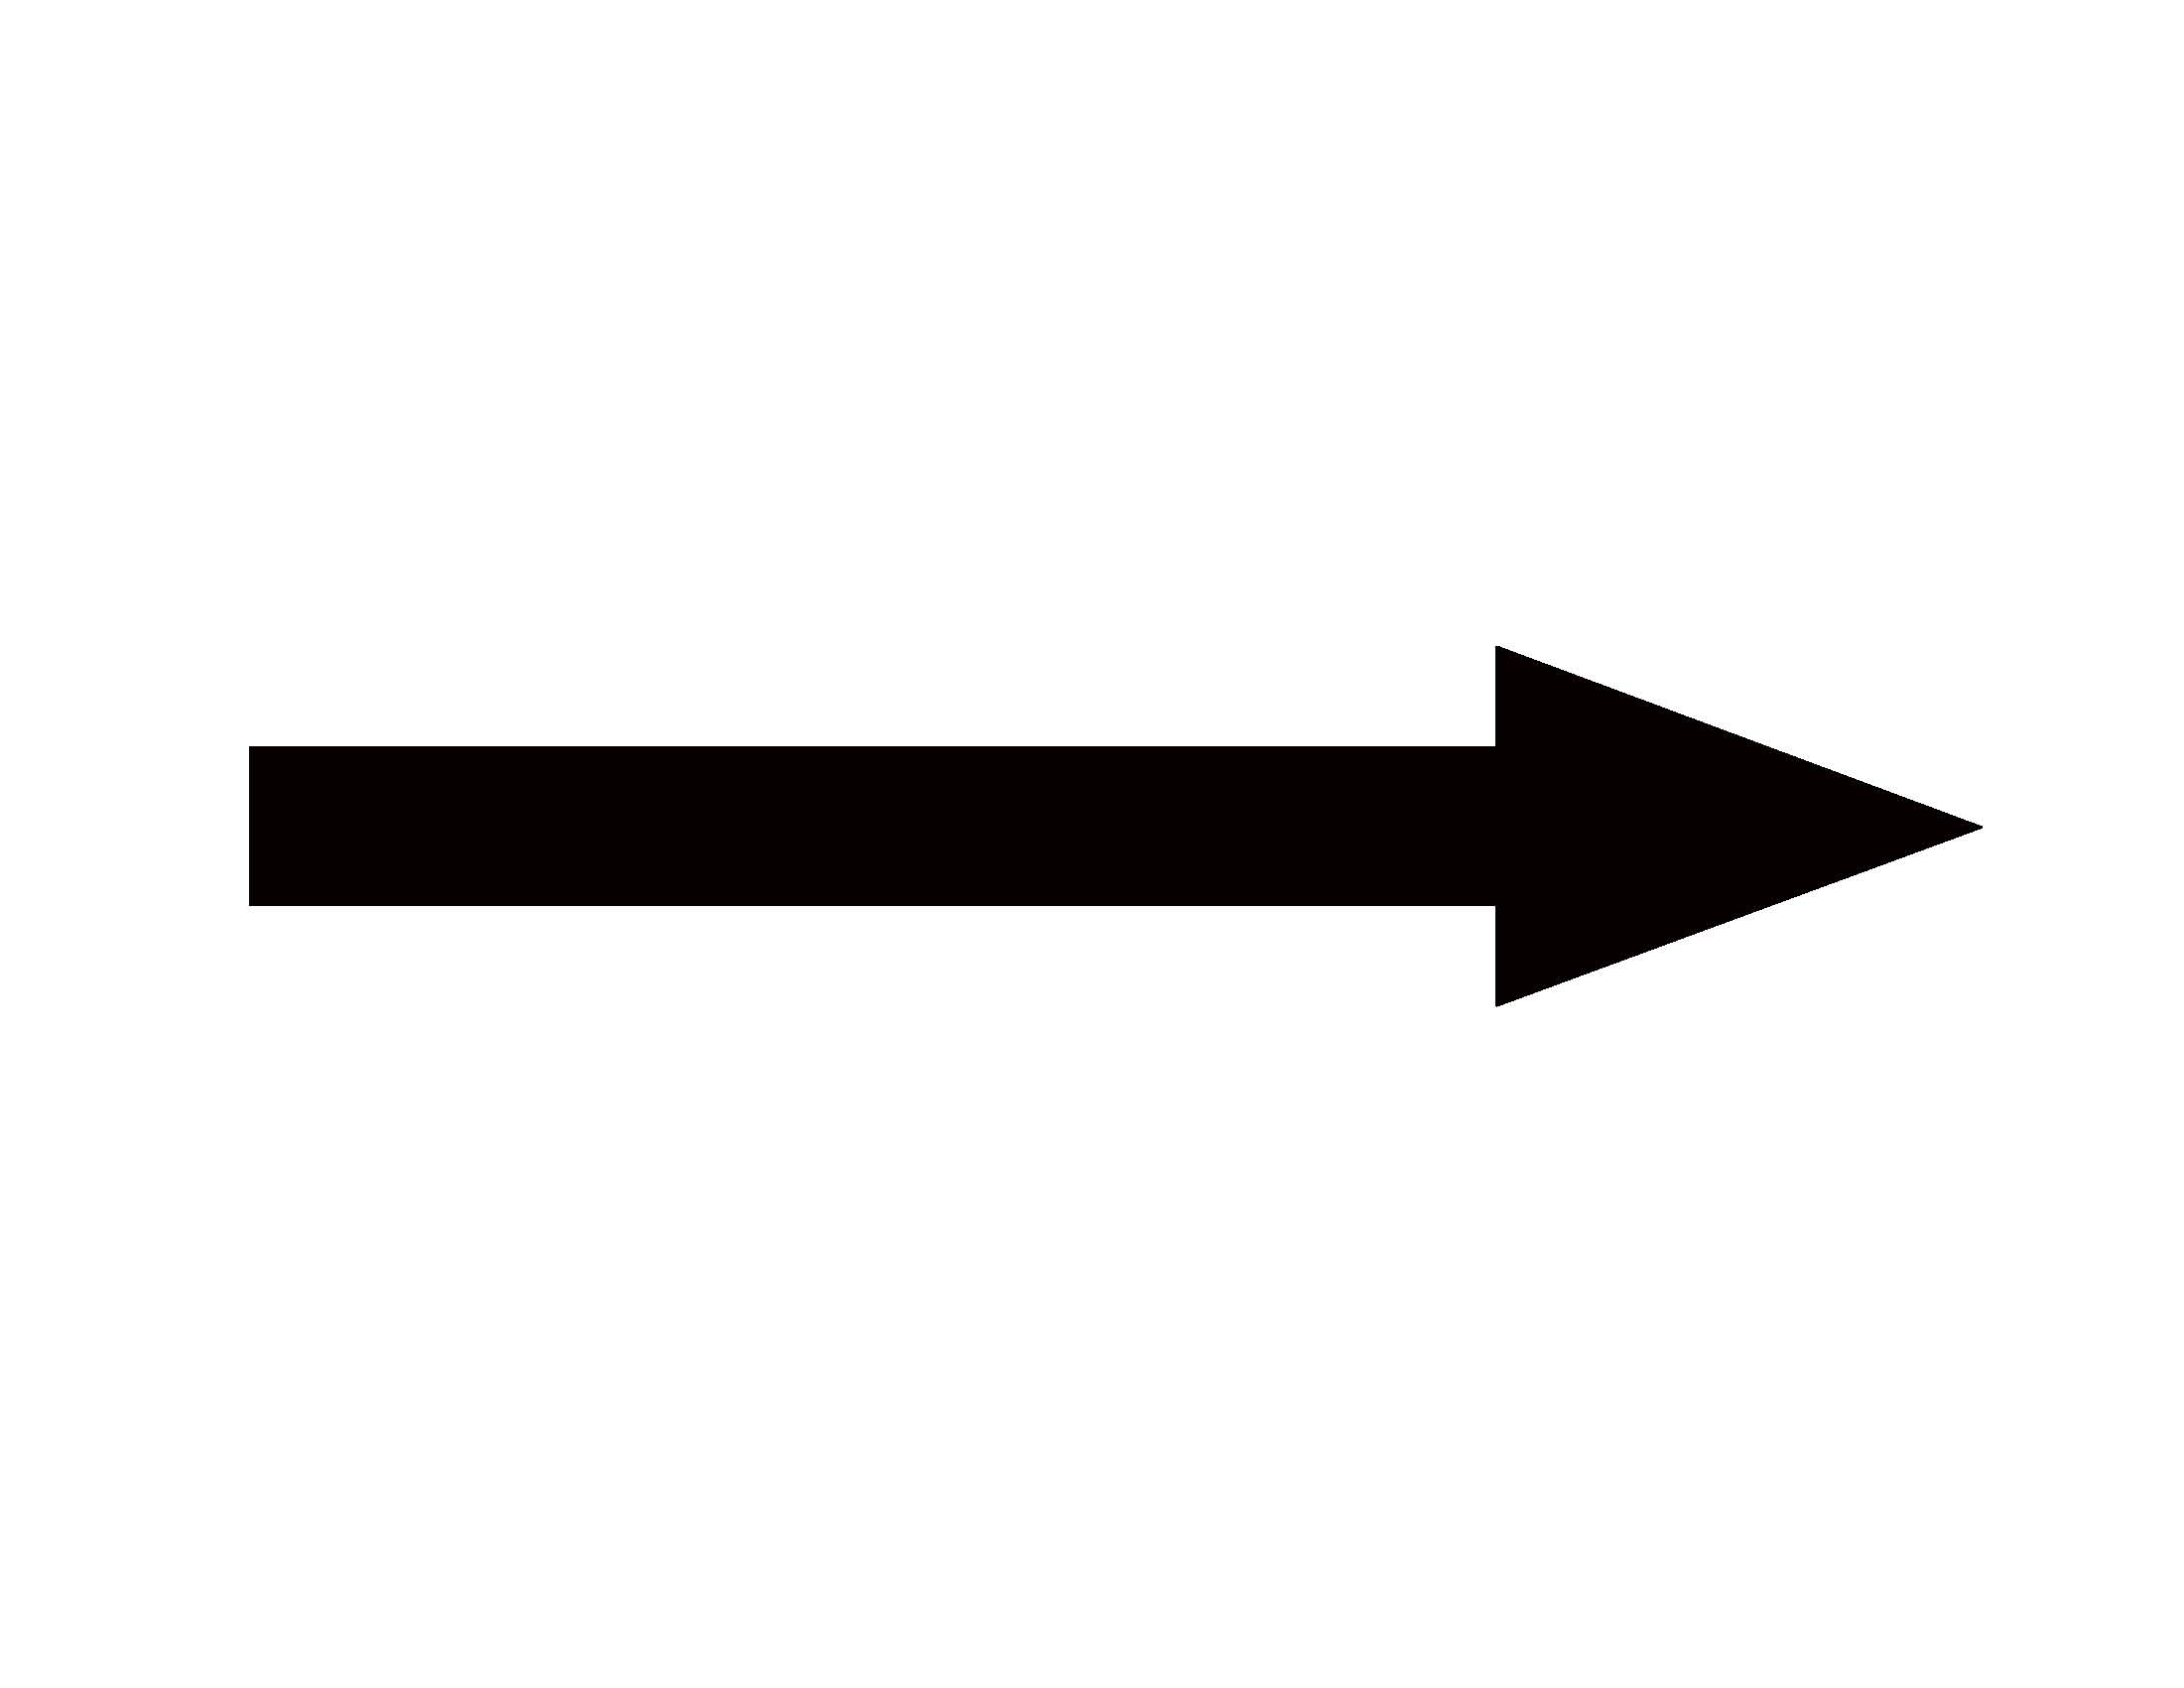
\includegraphics[width=\textwidth]{arrow.jpg}
                %% \caption{A tiger}
                %% \label{fig:tiger}
        \end{subfigure}
        ~ %add desired spacing between images, e. g. ~, \quad, \qquad, \hfill etc.
          %(or a blank line to force the subfigure onto a new line)
        \begin{subfigure}[c]{0.25\textwidth}
                
\includegraphics[width=\textwidth]{un_flag.png}
                %% \caption{A mouse}
                %% \label{fig:mouse}
        \end{subfigure}
        \caption{Flag Aggregation}
\end{figure}
\vfill
}

\frame{
  \frametitle{Background}

  Since the introduction of the new Statistical Working System (SWS),
  many innovative approaches has been devised to improve the current
  status and to accomodate for future needs of the fast changing world
  of statistics.

  \vfill

  One subtle yet fundamental change is the separation of a single
  symbol into two separate flag. A symbol or flag is a meta data which
  indicate the collection or methodological procedure that generates
  the value.

  \vfill

  The aim of this presentation is to introduce the change and how the
  observation status flag can impact future works.

}

\frame{
  \frametitle{Mixing of Status and Method}

  Historically, a symbol can represent how it was calculated, or where
  it was is collected. However, this mixed approach has created some
  confusion and loss of information.

  \vfill
  
  For example, when yield are calculated based on production and area
  harvested, a flag "C" representing "calculated" is
  assigned. However, it does not show the observation status of yield.

  \vfill

  A value for yield calculated based on official data has the same
  equivalent meaning to those calculated on estimates.

  \vfill

  This mixing of information results in loss of information and
  potential bias analysis.
  
 
}


\frame{
  \frametitle{Separation of Status and Method}

  To better represent these information, the decision was made to
  split the symbol into two separate flag reflecting different piece
  of information.

  \vfill

  One for the \textbf{observation status} which represents how the
  data was observed, whether collected from official or semi-official
  data source, or it maybe estimated or imputed.

  \vfill

  The second flag would denote the \textbf{methodology} it was
  obtained. Official figure can be obtained from questionnaire, or it
  can be from database or publications. Value which are estimated can
  be manually derived based or algorithm driven.

}


\frame{
  \frametitle{Problem}

  Nevertheless, it presents a problem. How do we assign observation
  flag when a value is calculated? Take the yield for example again,
  we would assign a method flag indicating the value was calculated;
  but what is its observation status?

  \vfill

  If we had production value collected from unofficial source (T)
  while area harvested were imputed (I), what is the observation flag
  for yield?
  
}


\section{Aggregation of Observation Flag}

\frame{
  \frametitle{What should the correct observation flag?}

  One approach is to quantify the quality of information for each flag
  and treating them as ordinal variables. Then the aggregation can be
  proceeded by taking the lower bounds of the set.

  %% Add in the mathematical representation
  \begin{block}{Flag Aggregation}
    $$
    F = \min_{\mathcal{S}}\left\{f_1, f_2, \cdots, f_n\right\}
    %% F = \left\{f: f, s \in \mathcal{S} \land f \le \forall s\right\}
    $$
  \end{block}
  Where the set $\mathcal{S}$ is the collection of flag which are used
  in the calculation.
  %% Where $f_i$ are all the flags used in the calculation
  \vfill

  The rational is that the aggregated flag should reflect the maximum
  amount of uncertainty.


}

\frame{
  \frametitle{The Flag Table}
  
  In order to take the minimum of the set, we will need to rank the
  flags.

  \vfill

  Shown below are subjective weights used to rank the flags.

  \begin{table}[h!]
    \begin{center}
      \caption{Description of the Observation flag}
      \begin{tabular}{|c|c|p{5cm}|}
        \hline
        Flags & Weights & Description\\
        \hline
        (blank) & 1 & Official Figure\\
        T & 0.8 & Unofficial figure\\
        E & 0.75 & Estimates\\
        I & 0.5 & Imputed\\
        M & 0 & Missing\\
        \hline
      \end{tabular}
    \end{center}  
  \end{table}
  

}


\frame{
  \frametitle{Example 1}
  
  Lets take the computation of yield for example again, if we had
  production value collected from unofficial source (T) while area
  harvested were imputed (I).

  \vfill

  Then provided with the previous table, we can compute the flag of
  yield as follow:
  
  \begin{block}{Flag Aggregation}
    $$
    \text{Flag of yield} = \min\left\{T, I\right\} = I
    $$
  \end{block}

}

\frame{
  \frametitle{Example 2}

  A second example arises in the case when we need to calculate
  regional aggregate.

  \vfill
  
  If we are trying to compute the total production of wheat of North
  America; with data from Canada and United States are unofficial (T) while
  the figure from Mexico is estimated (E).

  \vfill

  \begin{block}{Flag Aggregation}
    $$
    \text{Flag of aggregate} = \min\left\{T, E\right\} = E
    $$
  \end{block}



}




\section{Potential Applications}
\frame{
  \frametitle{}
  
  Flags have been collected for many decades, however, this piece of
  information have never been utilized.

  \vfill
  
  The recognition of various data source and quantification of the
  information quality provides many potential application which can
  enhance subsequent analysis.

}


\frame{
  \frametitle{Robust From Anormalies}
  %% include graphics on robust fitting

  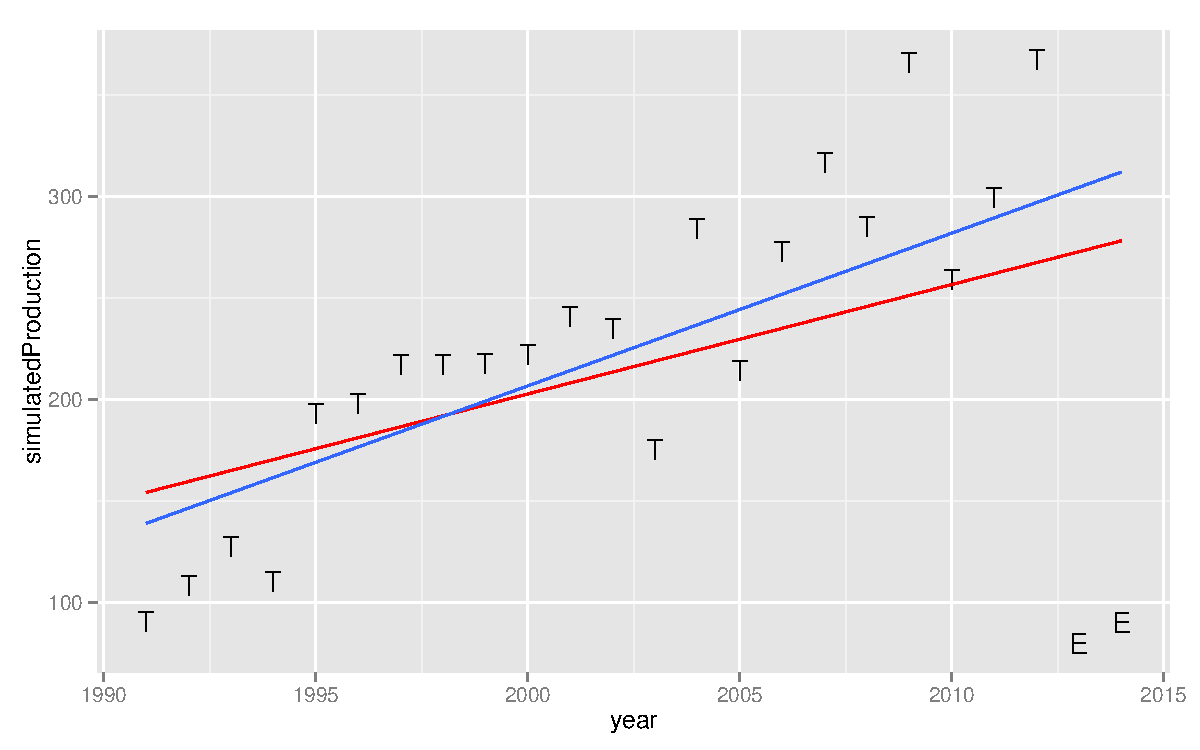
\includegraphics[scale=0.5]{robust.pdf}
}


\frame{
  \frametitle{Combining Source of Different Information Quality}
  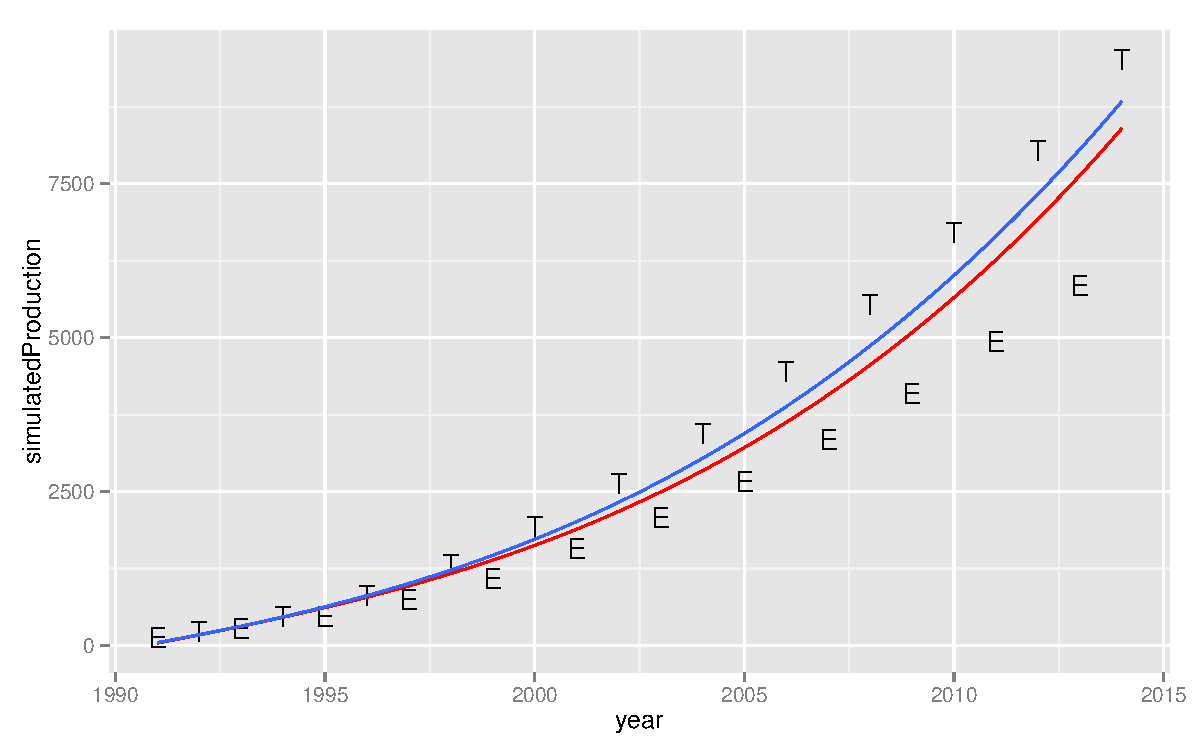
\includegraphics[scale=0.5]{combine.pdf}
  %% Include figure on combining different sources

}


\frame{
  \frametitle{}
  
  The potential associated with quantifying the quality of information
  is huge. It provides an additional piece of information for every
  single data point.

  \vfill
  
  This is a general framework, no specific methodology is required
  since any model and methodology can utilize this framework by
  incorporate the additional information.

}


\section{Computing Weights}


\frame{
  \frametitle{}

  Currently, the weights are assigned subjectively by expert
  judgements in order to preserve a rank order.

  \begin{table}[h!]
    \begin{center}
      \caption{Description of the Observation flag}
      \begin{tabular}{|c|c|p{5cm}|}
        \hline
        Flags & Weights & Description\\
        \hline
        (blank) & 1 & Official Figure\\
        T & 0.8 & Unofficial figure\\
        E & 0.75 & Estimates\\
        I & 0.5 & Imputed\\
        M & 0 & Missing\\
        \hline
      \end{tabular}
    \end{center}  
  \end{table}
  
  %% However, methods are being devised to estimate these weights
  %% objectively and automatically.

}


\frame{
  \frametitle{Objective Weights}
  
  A requirement for automatized and objective computation of weights
  is required due to the fact that we do not have the human resources
  to devote to assigning weights for each country, each agricultural
  domain and partition of the data.

}
  

\frame{
  \frametitle{Principle of Minimum Discrimination Information}

  Given derived information set, a new distribution $q$ should be
  chosen which is as hard to discriminate from the original
  distribution $p$ as possible; so that the new data produces as small
  an information gain as possible.

  \vfill

  In another word, the principle states that if we have to choose
  another representation, the information set which result in the
  least amount of information gain or uncertainty should be chosen.
  
}


\frame{
  \frametitle{Cross Entropy}

  \begin{block}{Cross-Entropy}
    \begin{align*}
    \mathrm{H}(P, Q) &=  \mathrm{H}(P) + D_{\mathrm{KL}}(P \| Q)\\
    \intertext{Where}
    H(P) &= -\sum_{i} {p(x_i) \log p(x_i)},\\
    D_{\mathrm{KL}}(P\|Q) &= \sum_i \log\left(\frac{p(i)}{q(i)}\right) p(i).\\
    \end{align*}
  \end{block}

}

\frame{
  \frametitle{Compute the weights}

  However, since the entropy of $H(x)$ would be the identical. We can
  simple calculate the Kullback-Leibler Divergence
  $D_{\mathrm{KL}}(P\|Q)$.

  \vfill
  After calculating the Kullback-Leibler Divergence, we can compute
  the weight according to the information gain.

  \vfill
  \begin{block}{Weights}
    $$
    \omega_i = \left\{
    \begin{array}{l r}
      1/(1 + D_{\mathrm{KL}}(P\|Q_i)) \quad \text{if $D_{\mathrm{KL}}(P\|Q_i) \ne 0$}\\
      1 - 1e^{-5} \, \, \, \, \quad \quad \quad \quad \quad \text{if $D_{\mathrm{KL}}(P\|Q_i) = 0$}
    \end{array} \right.
    $$
  \end{block}

  
}  


\frame{
  \frametitle{The New Flag Table}
  
  Shown below is the new set of weights for the wheat domain
  calculated based on the method above.

  \begin{table}[h!]
    \begin{center}
      \caption{New Observation Status Table of Wheat}
      \begin{tabular}{|c|c|p{5cm}|}
        \hline
        Flags & Weights & Description\\
        \hline
        (blank) & 1 & Official Figure\\
        T & 0.9901 & Unofficial Figure\\
        E & 0.97 & Estimates\\
        I &  & Imputed\\
        M & 0 & Missing\\
        \hline
      \end{tabular}
    \end{center}  
  \end{table}
  

}


\frame{
  \frametitle{The New Flag Table (Cont.)}
  

  \begin{table}[h!]
    \begin{center}
      \caption{New Observation Status Table of Ginger}
      \begin{tabular}{|c|c|p{5cm}|}
        \hline
        Flags & Weights & Description\\
        \hline
        (blank) & 1 & Official Figure\\
        T & 0.943 & Unofficial Figure\\
        E & 0.873 & Estimates\\
        I &  & Imputed\\
        M & 0 & Missing\\
        \hline
      \end{tabular}
    \end{center}  
  \end{table}
  

}

\frame{
  \frametitle{Concusion}
  
  We hope this new change and framework will assist users to improve
  their work and utilize information which has been collected over
  several decades.
  
}



%% \frame{
%%   \frametitle{Benford's Law}

%%   In the previous approach, we took the official figures as the
%%   benchmark. Nevertheless, we may want to know how it compares to the
%%   true distribution.
  
%%   \vfill

%%   For large commodities, we can potentially use the \textbf{Benford
%%   distribution} or the \textbf{First-Digit Law}.
  
%%   \begin{block}{Benford Distribution}
%%     $$
%%     P(d)=\log_{10} \left(1+\frac{1}{d}\right).
%%     $$
%%   \end{block}

%%   Then we can calculate the Kullback-Leibler Divergence with respect
%%   to the Benford Distribution.
  

%% }



%% \frame{

%%   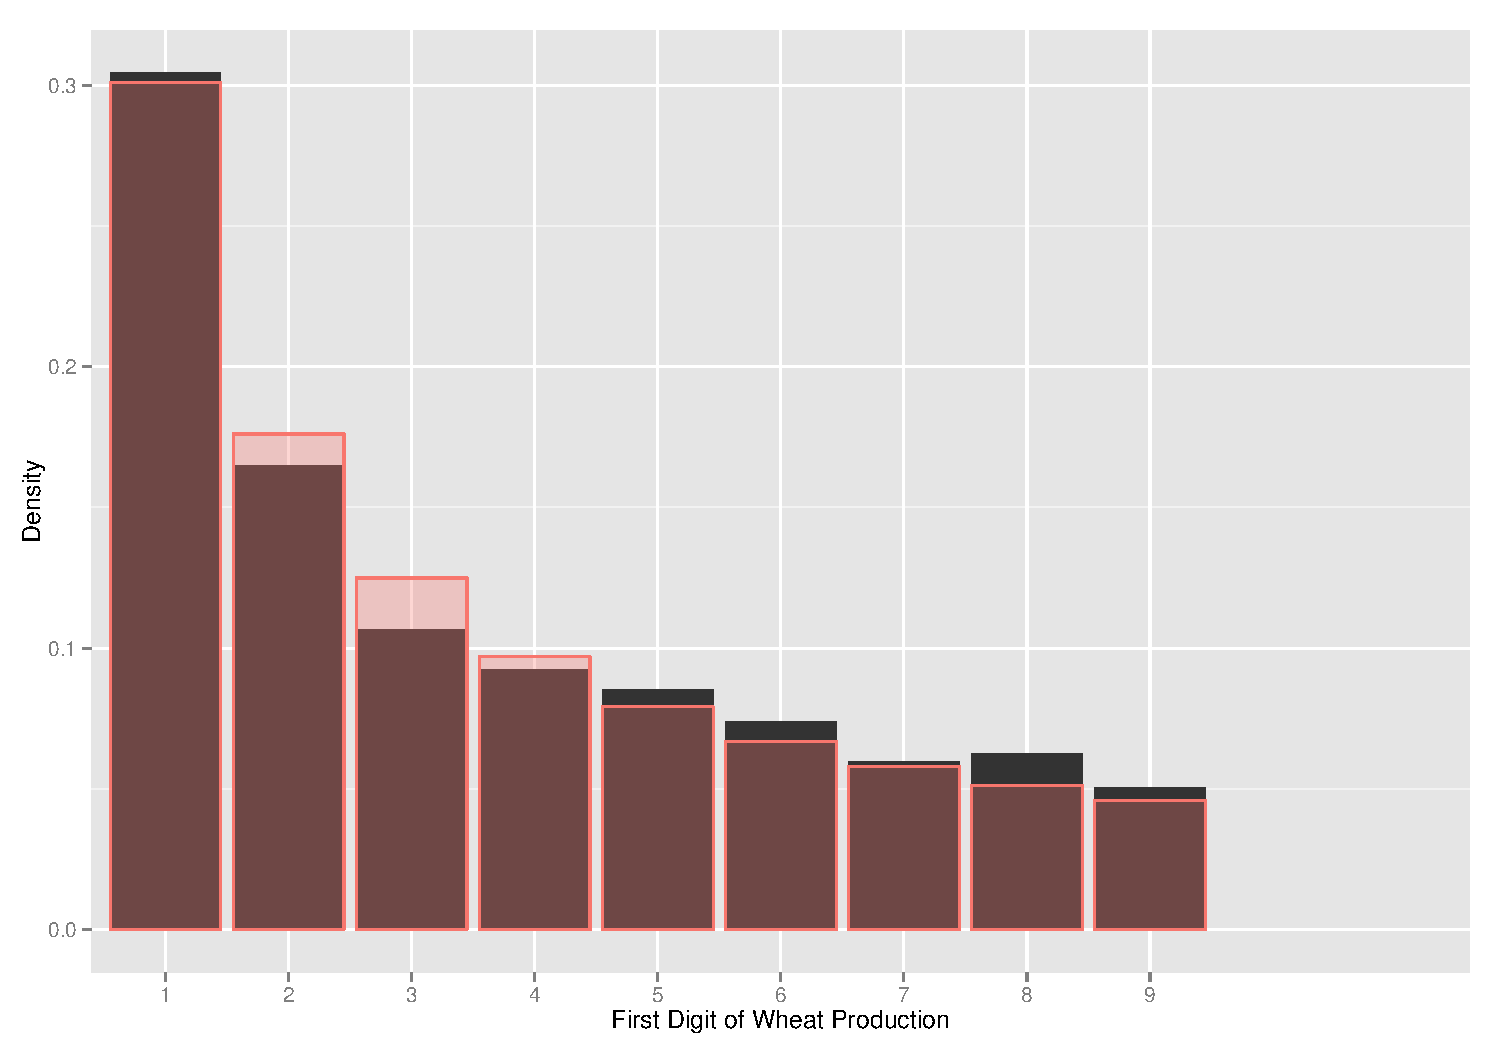
\includegraphics[scale = 0.45]{benford}

%% }


%% See if we can use AIC

%% \frame{
%%   \frametitle{Self-Similarity Weights}

%%   In this approach, we try to estimate the true value based on
%%   similarity. The rational is that since all different sources are
%%   intended to measure the same value, the true value should be within
%%   the cluster of the observed points. Then the centroid is used as an
%%   approximation to the true value.
  
%%   \vfill

%%   The distance from the centroid will be inversely related to the
%%   weight. That is, the further away you are from the centroid, the
%%   lower the weight will be assigned.
  
%% }

%% \frame{
%%   \centering
%%   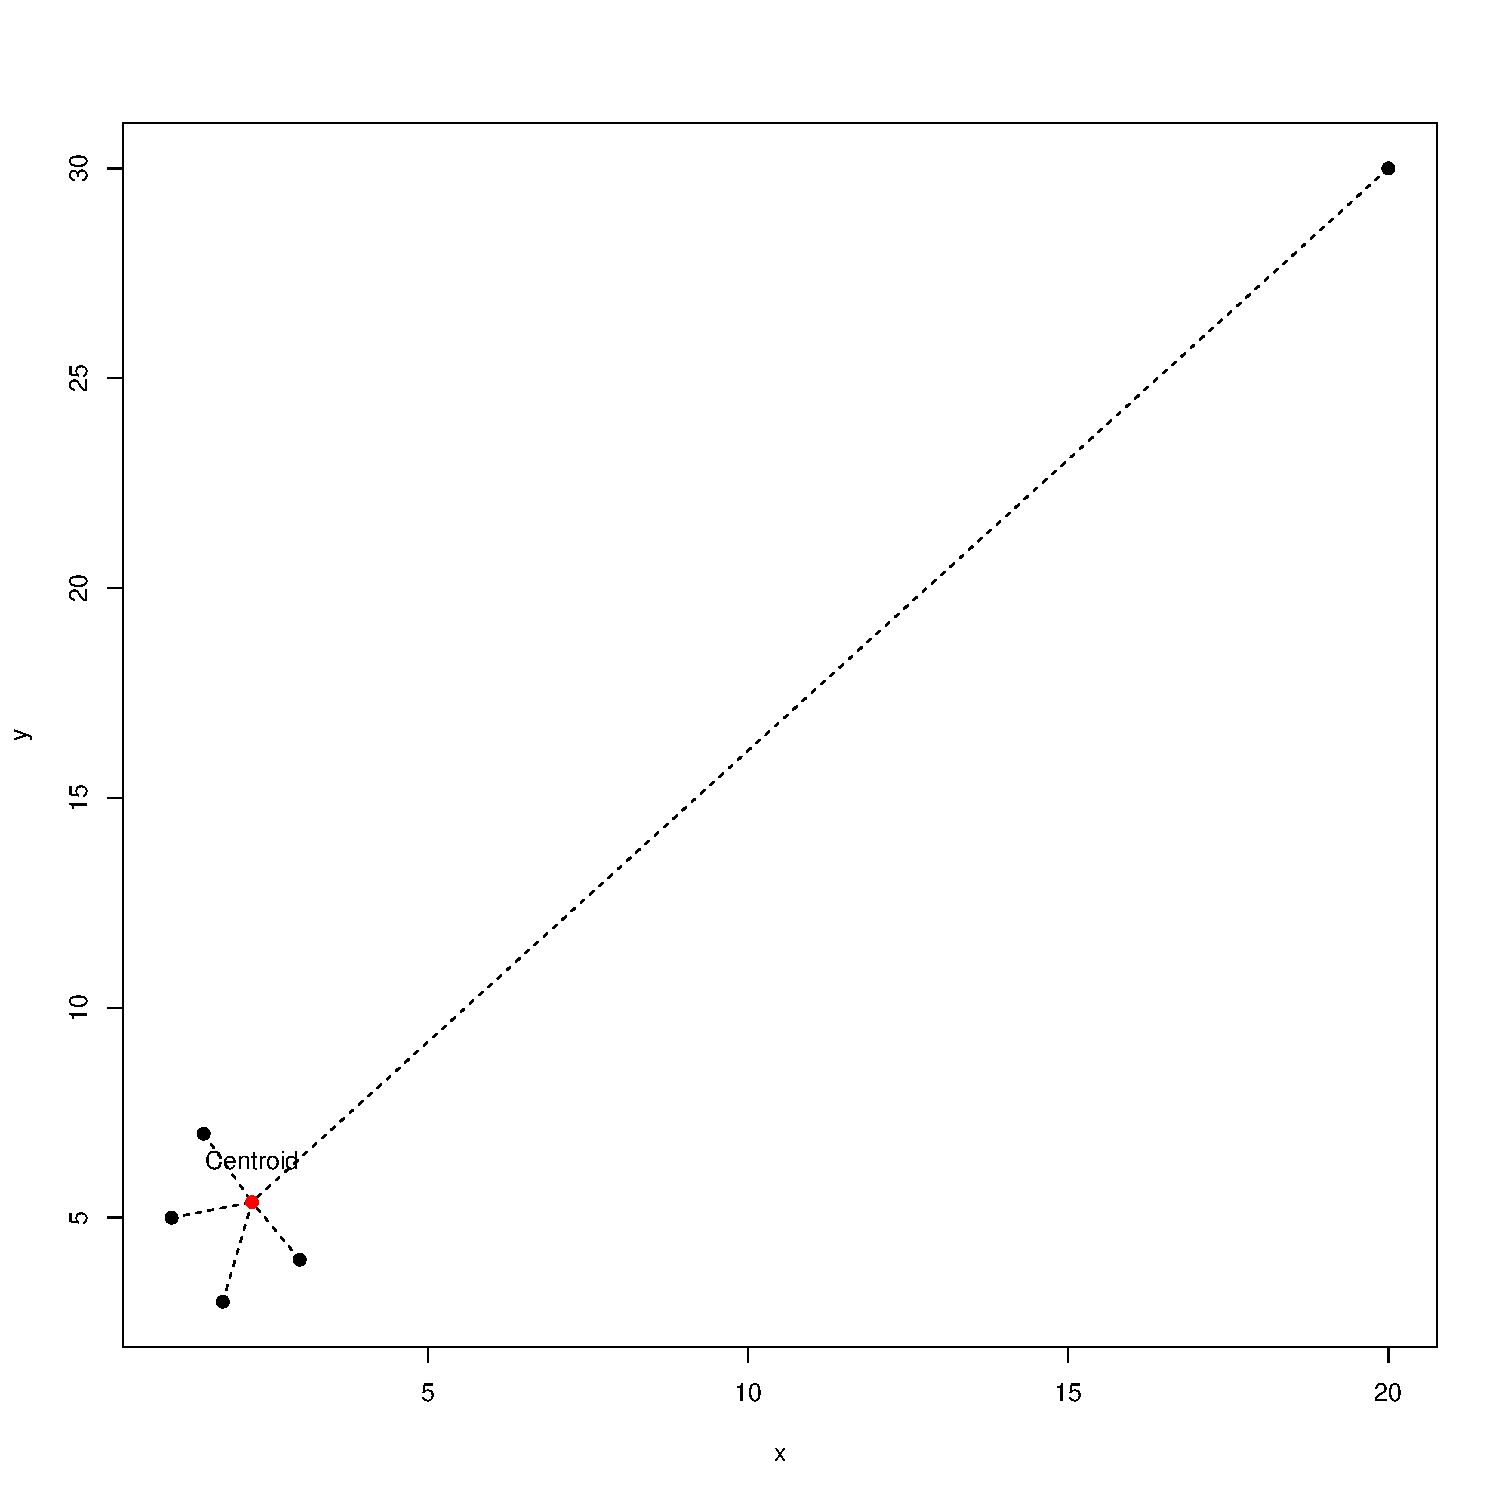
\includegraphics[scale=0.3]{centroid.pdf}
  
%% }  


\end{document}
